% -*- mode: latex; mode: flyspell; ispell-local-dictionary: "en_US"; coding: utf-8; fill-column: 80 -*-

\documentclass{article}

\usepackage[utf8]{inputenc}
\usepackage[english]{babel}

\usepackage{amsmath,amsfonts,amssymb}
\usepackage{fullpage}
\usepackage{verbatim}

\usepackage{tikz,pgfplots}

\pgfplotsset{
  width=150mm,height=100mm,
  major grid style={thin,dotted,color=black!50},
  minor grid style={thin,dotted,color=black!50},
  grid,
  every axis/.append style={
    line width=0.5pt,
    tick style={
      line cap=round,
      thin,
      major tick length=4pt,
      minor tick length=2pt,
    },
  },
  legend cell align=left,
  legend pos=north west,
}

%%%%%%%%%%%%%%%%%%%%%%%%%%%%%%%%%%%%%%%%%%%%%%%%%%%%%%%%%%%%%%%%%%%%%%%%%%%%%%%%

\begin{document}

\title{Hashmap Sizes}
\author{}
\maketitle


% IMPORT-DATA mphf stats_mphf_size.txt


\begin{center}
	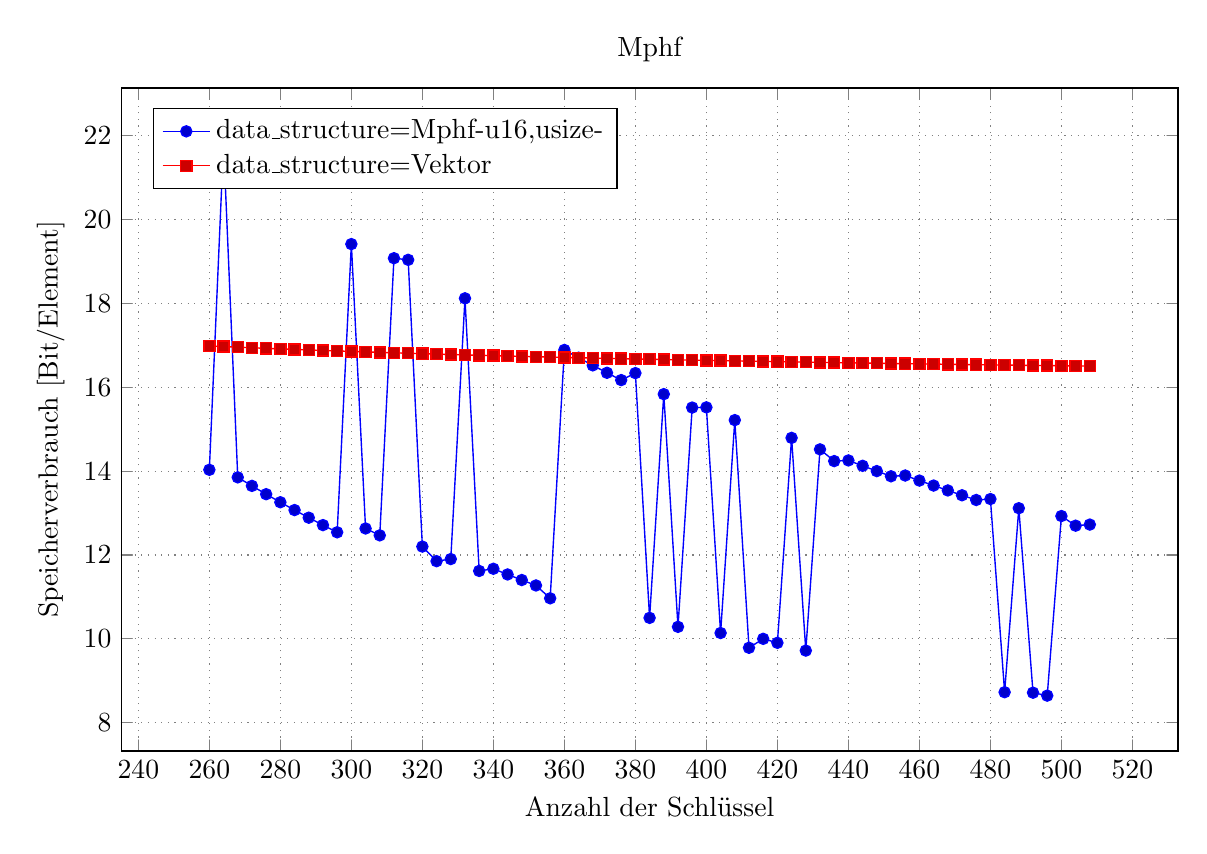
\begin{tikzpicture}
	\begin{axis}[
	title={Mphf},
	xlabel={Anzahl der Schlüssel},
	ylabel={Speicherverbrauch [Bit/Element]},
	]
	
	%% MULTIPLOT(data_structure) SELECT size AS x, size_bytes AS y, MULTIPLOT
	%% FROM mphf WHERE x % 4 == 0 AND x > 256 AND x < 512 GROUP BY MULTIPLOT,x ORDER BY MULTIPLOT,x
 \addplot coordinates { (260,14.0308) (264,21.8182) (268,13.8507) (272,13.6471) (276,13.4493) (280,13.2571) (284,13.0704) (288,12.8889) (292,12.7123) (296,12.5405) (300,19.4133) (304,12.6316) (308,12.4675) (312,19.0769) (316,19.038) (320,12.2) (324,11.8519) (328,11.9024) (332,18.1205) (336,11.619) (340,11.6706) (344,11.5349) (348,11.4023) (352,11.2727) (356,10.9663) (360,16.8889) (364,16.7033) (368,16.5217) (372,16.3441) (376,16.1702) (380,16.3368) (384,10.5) (388,15.8351) (392,10.2857) (396,15.5152) (400,15.52) (404,10.1386) (408,15.2157) (412,9.78641) (416,10.0) (420,9.90476) (424,14.7925) (428,9.71963) (432,14.5185) (436,14.2385) (440,14.2545) (444,14.1261) (448,14.0) (452,13.8761) (456,13.8947) (460,13.7739) (464,13.6552) (468,13.5385) (472,13.4237) (476,13.3109) (480,13.3333) (484,8.72727) (488,13.1148) (492,8.71545) (496,8.64516) (500,12.928) (504,12.6984) (508,12.7244) };
 \addlegendentry{data\_structure=Mphf-u16,usize-};
 \addplot coordinates { (260,16.9846) (264,16.9697) (268,16.9552) (272,16.9412) (276,16.9275) (280,16.9143) (284,16.9014) (288,16.8889) (292,16.8767) (296,16.8649) (300,16.8533) (304,16.8421) (308,16.8312) (312,16.8205) (316,16.8101) (320,16.8) (324,16.7901) (328,16.7805) (332,16.7711) (336,16.7619) (340,16.7529) (344,16.7442) (348,16.7356) (352,16.7273) (356,16.7191) (360,16.7111) (364,16.7033) (368,16.6957) (372,16.6882) (376,16.6809) (380,16.6737) (384,16.6667) (388,16.6598) (392,16.6531) (396,16.6465) (400,16.64) (404,16.6337) (408,16.6275) (412,16.6214) (416,16.6154) (420,16.6095) (424,16.6038) (428,16.5981) (432,16.5926) (436,16.5872) (440,16.5818) (444,16.5766) (448,16.5714) (452,16.5664) (456,16.5614) (460,16.5565) (464,16.5517) (468,16.547) (472,16.5424) (476,16.5378) (480,16.5333) (484,16.5289) (488,16.5246) (492,16.5203) (496,16.5161) (500,16.512) (504,16.5079) (508,16.5039) };
 \addlegendentry{data\_structure=Vektor};
 
	
	\end{axis}
	\end{tikzpicture}
\end{center}


\end{document}

%%%%%%%%%%%%%%%%%%%%%%%%%%%%%%%%%%%%%%%%%%%%%%%%%%%%%%%%%%%%%%%%%%%%%%%%%%%%%%%%
